\section{Image formation}
\label{sec:img_formation}
\begin{itemize}
	\item To fully understand/analyze an image, we first have to examine how it was created (note that an image is a 2D representation of a 3D world)
	\item Various challenges occur in CV 
	\begin{figure}[ht!]
		\centering
		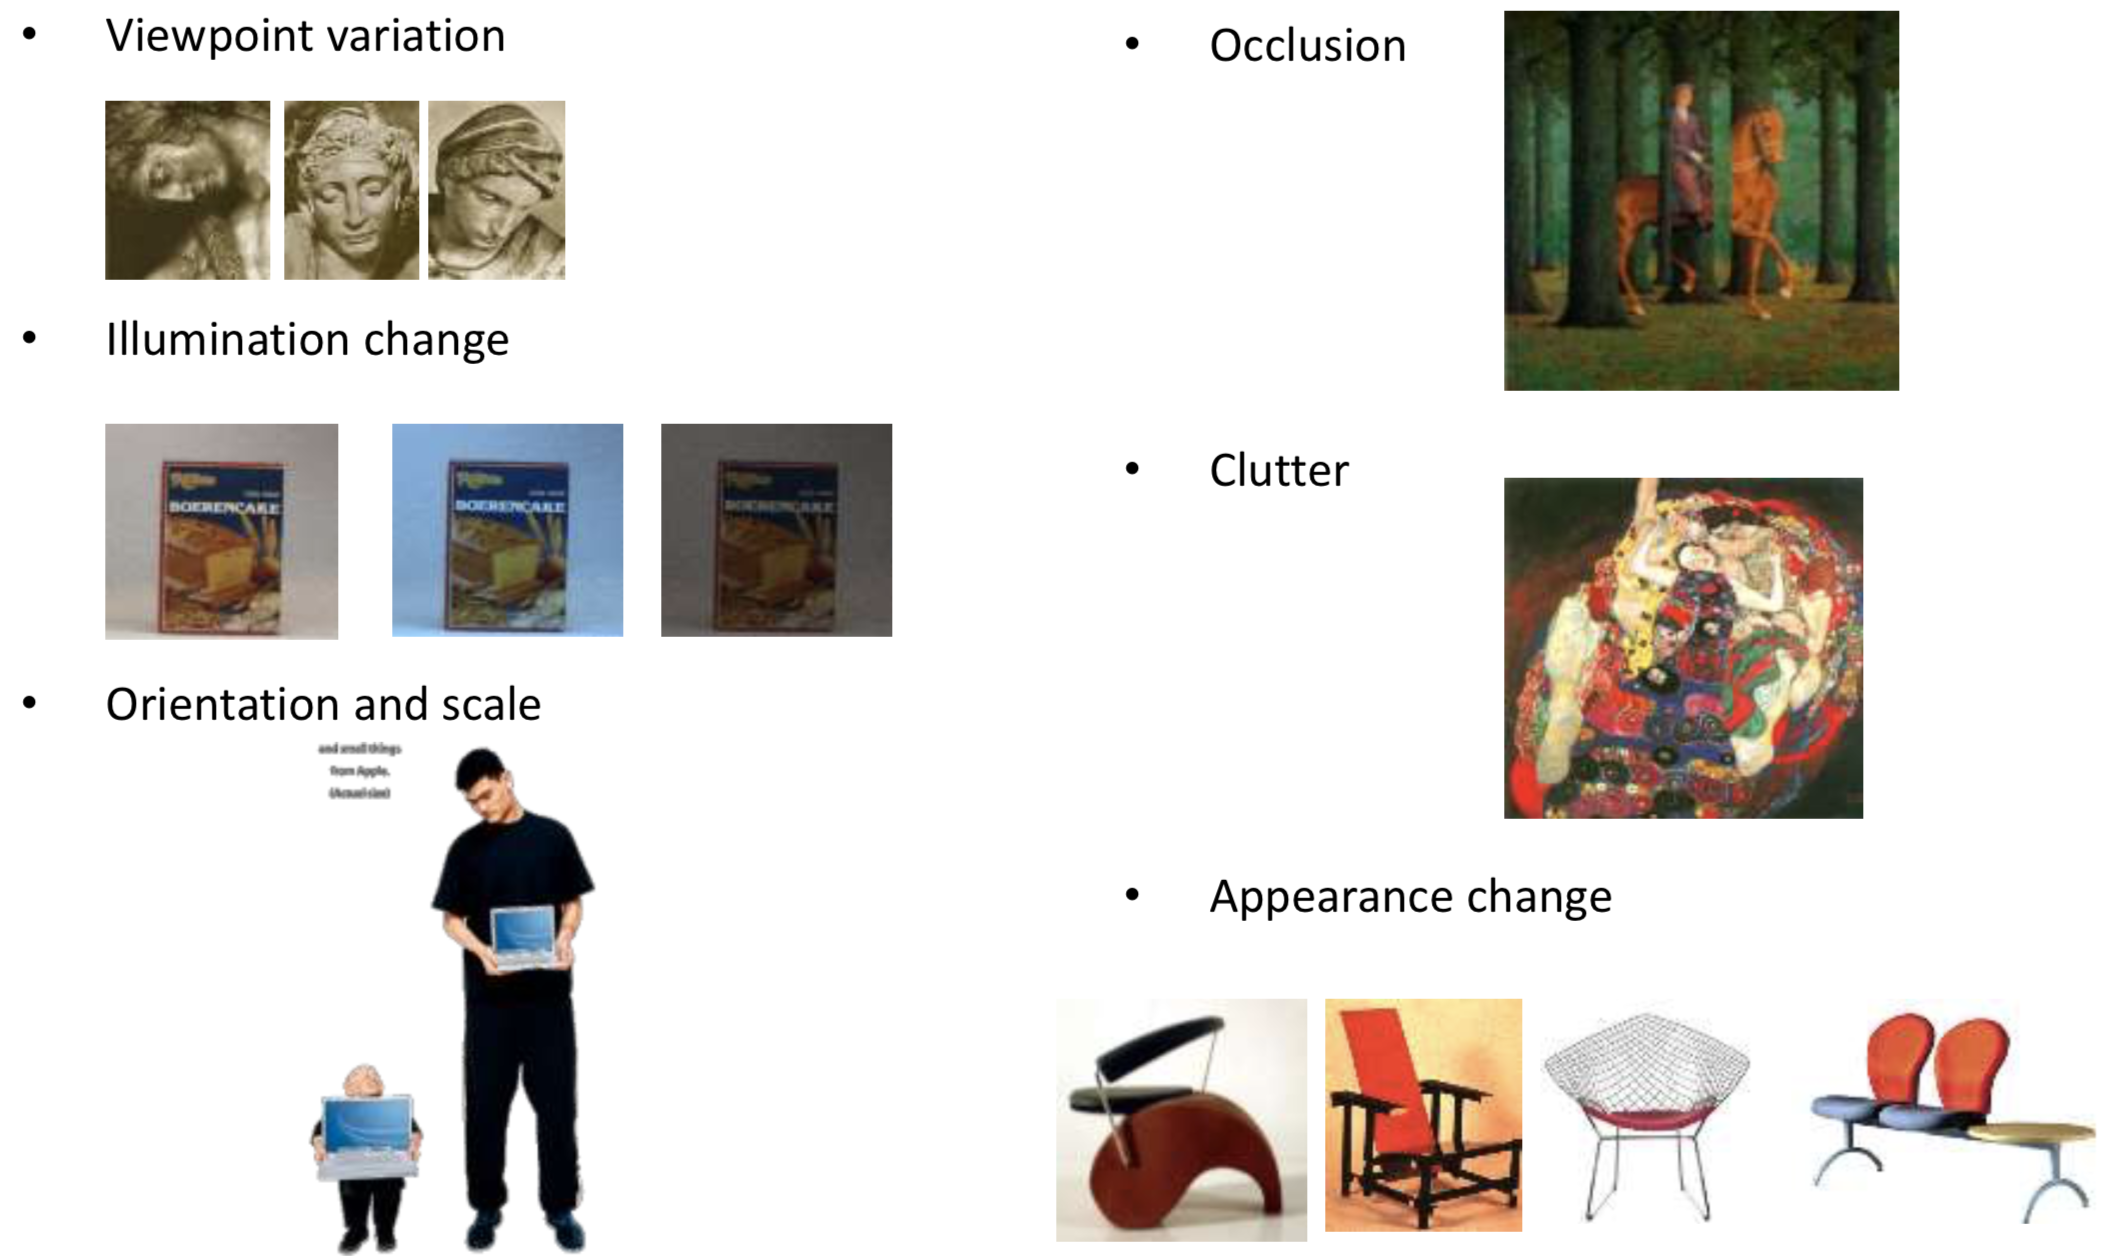
\includegraphics[width=0.5\textwidth]{figures/cv_image_formation_challenges_cv.png}
		\caption{Challenges in Computer Vision}
	\end{figure}
	\item The two main parts of how an image is formed are:
	\begin{itemize}
		\item \textit{Geometry} of the projection of a 3D environment to a 2D image. This defines which pixel belongs to which object (part/location). 
		\item \textit{Physics of light} which determines the brightness of a point in the image plane as a function of illumination and surface properties. Thus, the light source has a crucial influence on an object's appearance 
	\end{itemize}
\end{itemize}
\subsection{Projective Geometry and Camera models}
\begin{itemize}
	\item A camera can be abstracted by a pinhole model. Larger aperture/pinhole results in blurry images, smaller give sharp but noisy images (less energy of light is being passed) $\Rightarrow$ Change between both by using different lenses
	\item We represent an image by a projection plane. The intersection between the center of projection and the plane is determined by (note that $z$ is negative):
	$$(x,y,z)\to (-\frac{d}{z}\cdot x, -\frac{d}{z}\cdot y, -d)$$ 
	\begin{figure}[ht!]
		\centering
		\begin{subfigure}[b]{0.48\textwidth}
			\centering
			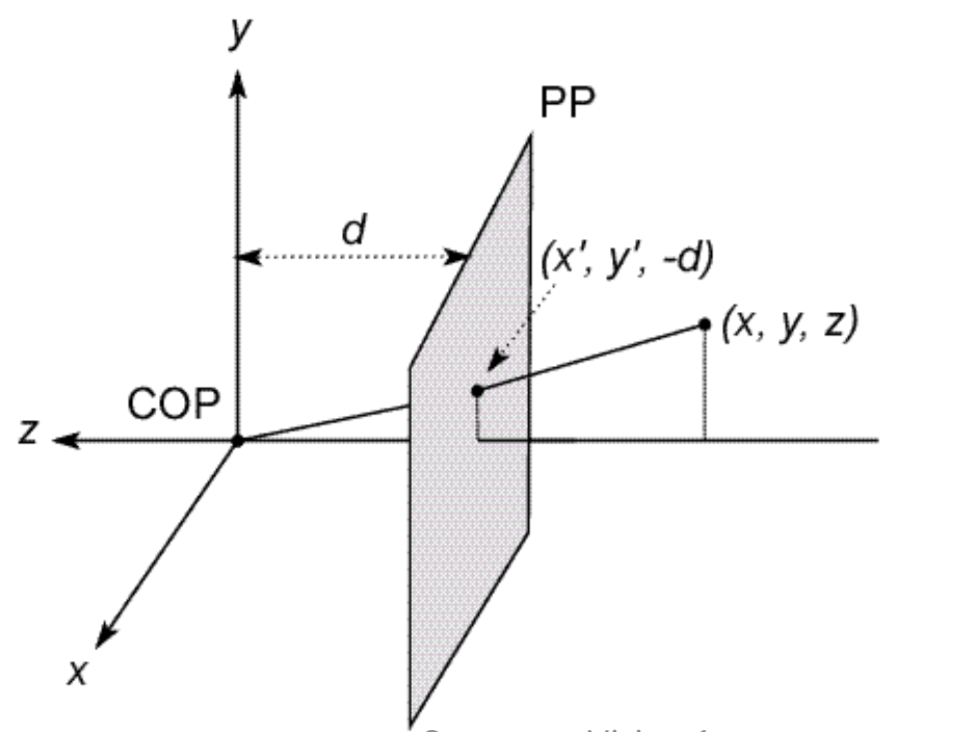
\includegraphics[width=0.4\textwidth]{figures/cv_image_formation_3D_model.png}
			\caption{Projection plane}
		\end{subfigure}
		\begin{subfigure}[b]{0.48\textwidth}
			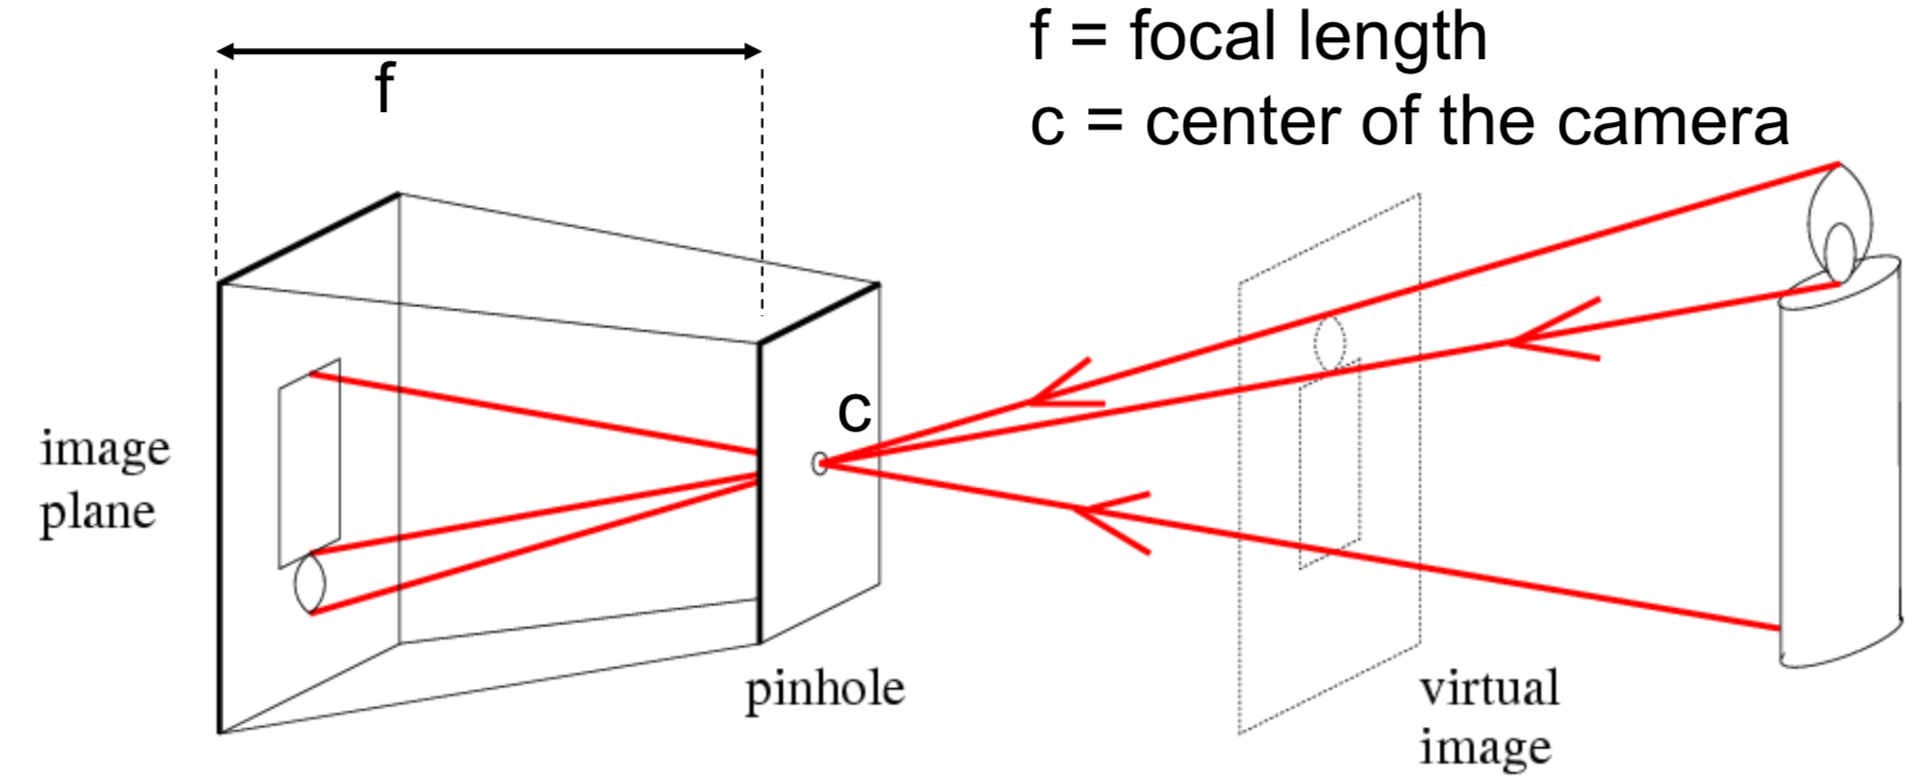
\includegraphics[width=0.8\textwidth]{figures/cv_image_formation_3D_model_2.png}
			\caption{Pinhole camera model}
		\end{subfigure}
		\caption{Abstract camera model in 3D coordinates}
	\end{figure}
	\item Model projection of 3D points to 2D image plane using homogeneous coordinates. The components we use for the projection are:
	\begin{itemize}
		\item \textit{Viewport projection}: Convert plane points to image coordinates (top left corner $(0,0)$, resolution scaling $s_x$, $s_y$)
		\item \textit{Perspective projection}: 3D points to image plane (homogeneous coordinates)
		\item \textit{View transformation}: rotation and translation matrix $\bm{R}$ and $\bm{T}$ for modeling the position and orientation of the camera. Can be seen as changing the coordinate system
		\item All together, we get the transformed points by:
		$$\left[\begin{array}{c}u\\v\\1\end{array}\right] = \underbrace{\left[\begin{array}{ccc}s_x & 0 & u_0\\0 & -s_y & v_0\\0 & 0 & 1\end{array}\right]}_{\text{Viewport}} \cdot \underbrace{\left[\begin{array}{cccc}1 & 0 & 0 & 0\\0 & 1 & 0 & 0\\0 & 0 & -1/d & 0\end{array}\right]}_{\text{Perspective}} \cdot \underbrace{\left[\begin{array}{cc}\bm{R} & \bm{T} \\\bm{0}^T_3 &  1\end{array}\right]}_{\text{View}} \cdot \left[\begin{array}{c}x\\y\\z\\1\end{array}\right]$$
	\end{itemize}
	\item Viewport and perspective projection depend on the camera (size and position of image plain) so that those are called \textit{intrinsic} camera parameter. In contrast, the view transformation is determined by \textit{extrinsic} camera parameters as it defines the camera position in the (original) coordinate system
\end{itemize}
\subsection{Light and Color models}
\label{sec:color_models}
\begin{itemize}
	\item The appearance color of an object is influenced by three components
	\begin{itemize}
		\item \textit{Light source}: spectral power distribution of light $e(\lambda)$ 
		\item \textit{Object}: the reflection distribution of an object $p(\lambda)$ (how good certain wavelengths are reflected)
		\item \textit{Sensor}: Detection by the sensor of the distribution $e(\lambda) p(\lambda)$
	\end{itemize}
	\item The goal is to be invariant to light source $e(\lambda)$ and sensor perspective
	\item Two very simple approaches to make an image independent of light source
	\begin{itemize}
		\item \textbf{Gray-world} assumption: the world is in average gray. So, we rescale every channel independently by $128/$mean of channel. Problematic if image is biased towards not being grey (high single channel, etc.)
		\item \textbf{Scale-by-max}/\textbf{White-patch} assumption: there is always at least one white pixel in an image. Hence, the channels are rescaled by $255$/max of channel. Fails if there is actually no white pixel in the image (results in wrong maximum), or if white pixel is in the shadow $\Rightarrow$ assumes whole image being shaded.
		\item All models underly/use the von Kries model where we convert an unknown light source $u$ to a canonical $c$ (i.e. day light) by simple channel scaling:
		$$\left(\begin{array}{c}R^c\\G^c\\B^c\end{array}\right) = \left(\begin{array}{ccc}
		\alpha & 0 & 0 \\
		0 & \beta & 0\\
		0 & 0 & \gamma
		\end{array}\right) \cdot \left(\begin{array}{c}R^u\\G^u\\B^u\end{array}\right)$$
		Note that to simplify the calculation of $\alpha$, $\beta$ and $\gamma$, and assume that the channels $R$, $G$ and $B$ are independent (thus only diagonal matrix), we approximate the integral as single wavelength for narrow-band filters.
	\end{itemize}
	\item As computer can't handle continuous distributions, the following integrals are approximate by for example the RGB model:
	$$R = \int_\lambda e(\lambda) p(\lambda) f_R(\lambda) d\lambda, \hspace{2mm}G = \int_\lambda e(\lambda) p(\lambda) f_G(\lambda) d\lambda, \hspace{2mm}B = \int_\lambda e(\lambda) p(\lambda) f_B(\lambda) d\lambda$$
	Every spectral color (see below diagram in Figure~\ref{fig:rgb_color_wavelength_distribution_RGB}) can be represented by an linear combination of RGB values.
	Note that human ganglion cells have similar functions, but are the most sensitive to green.
	\begin{figure}[ht!]
		\centering
		\begin{subfigure}[b]{0.4\textwidth}
			\centering
			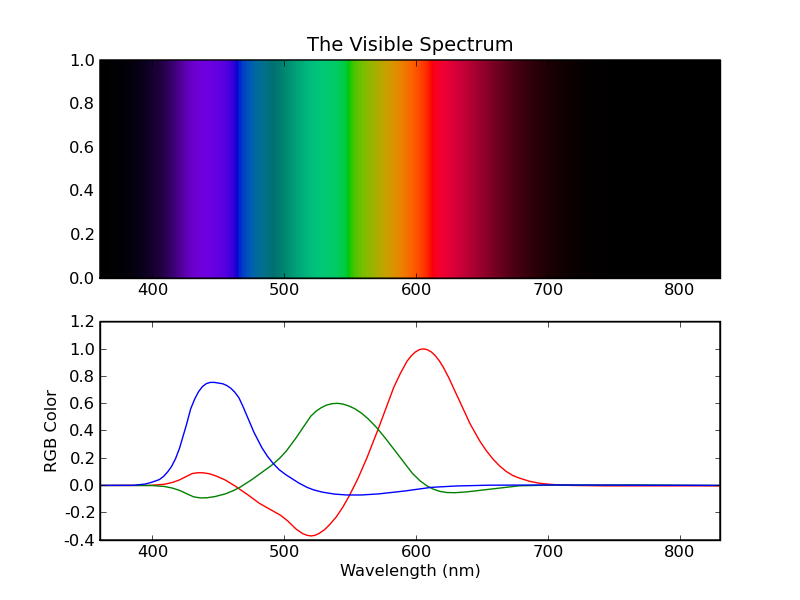
\includegraphics[width=0.75\textwidth]{figures/cv_image_formation_color_RGB_model.png}
			\caption{RGB model}
			\label{fig:rgb_color_wavelength_distribution_RGB}
		\end{subfigure}
		\begin{subfigure}[b]{0.24\textwidth}
			\centering
			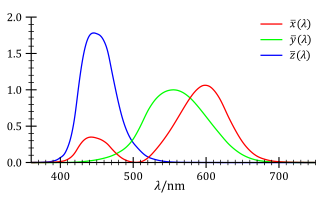
\includegraphics[width=\textwidth]{figures/cv_image_formation_color_XYZ_model.png}
			\caption{XYZ model}
			\label{fig:rgb_color_wavelength_distribution_XYZ}
		\end{subfigure}
		\hspace{5mm}
		\begin{subfigure}[b]{0.28\textwidth}
			\centering
			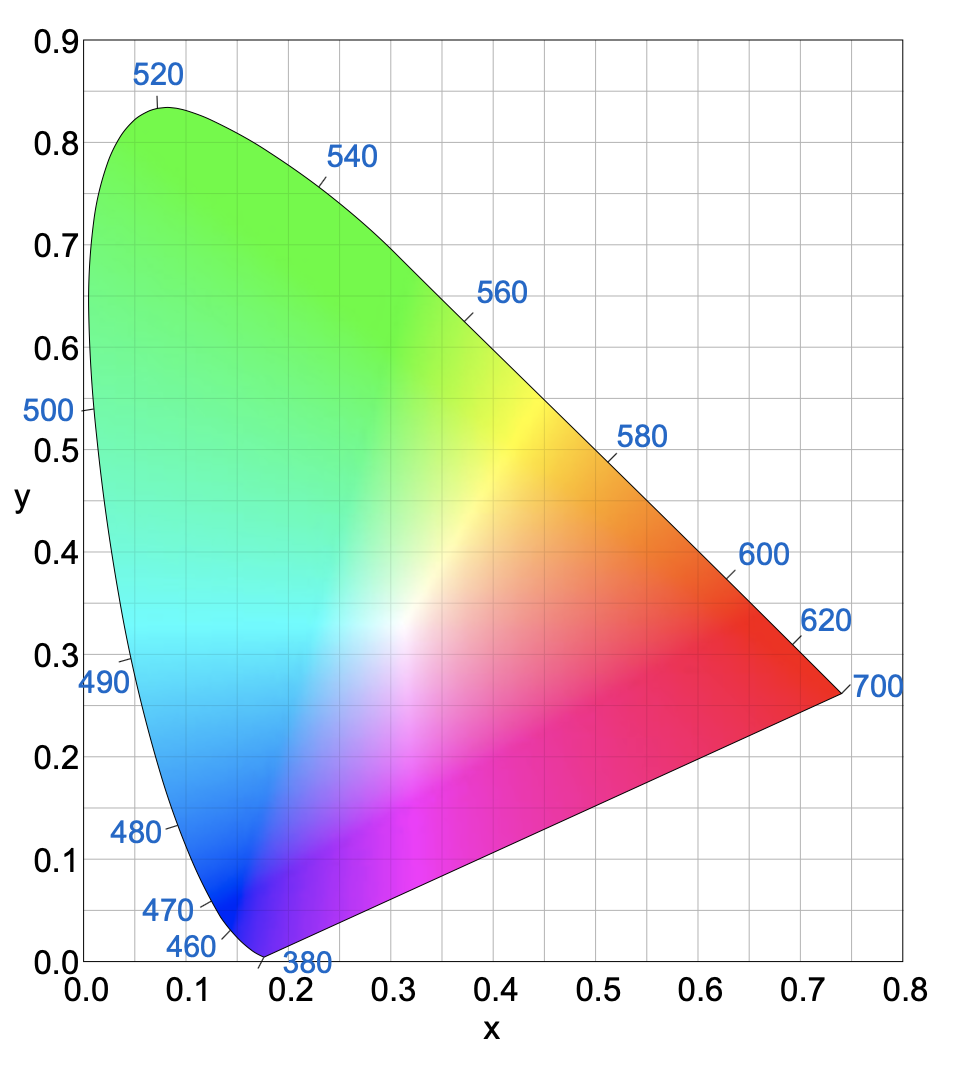
\includegraphics[width=0.8\textwidth]{figures/cv_image_formation_color_XYZ_diagram_2.png}
			\caption{XYZ diagram}
			\label{fig:rgb_color_wavelength_distribution_XYZ_diagram}
		\end{subfigure}
		\caption{Color matching functions $f_R$, $f_G$ and $f_B$ for the standard (a) RGB / (b) XYZ model. The colors represented by the XYZ system are shown in (c). Note that the line of purples contains colors that cannot be created by a monochromatic light source and needs a combination of fully saturated red and violet (max and min of spectrum).}
		\label{fig:rgb_color_wavelength_distribution}
	\end{figure}
	\item The intensity of the RGB color space is calculated by the sum of the channels: $I=R+G+B$
	\item Another color space is the XYZ system. The color matching functions $\overline{x}(\lambda), \overline{y}(\lambda), \overline{z}(\lambda)$ are similar but not the same as RGB (see Figure~\ref{fig:rgb_color_wavelength_distribution_XYZ}). The values are calculated by:
	$$X = \int_\lambda e(\lambda) p(\lambda) \overline{x}(\lambda) d\lambda, \hspace{2mm}Y = \int_\lambda e(\lambda) p(\lambda) \overline{y}(\lambda) d\lambda, \hspace{2mm}Z = \int_\lambda e(\lambda) p(\lambda) \overline{z}(\lambda) d\lambda$$
	\item However, we can split these measurements into a brightness/luminance and chromaticity/color component specified by $x$ and $y$. The luminance is given by $Y$ ($XYZ$ was designed for that), and the chromaticity is determined as ($Z$ is implicitly given by $1-x-y$):
	$$x=\frac{X}{X+Y+Z},\hspace{2mm}y=\frac{Y}{X+Y+Z}$$
	\item The created colors can be visualized in an $xy$-diagram (see Figure~\ref{fig:rgb_color_wavelength_distribution_XYZ_diagram}). 
	\item Given a reference light source $e$, we can determine the dominant wavelength (\textit{hue}) of a point $p$ by a line from $e$ through $p$ towards the boundary. The \textit{saturation} is given by the ratio of line length between $e$ and $p$ and $e$ to dominant wavelength boundary. Combining these with the luminance $Y$, a point $p$ can be converted into the HSI color space (see Figure~\ref{fig:rgb_color_HSV_color_cone}).
	\item HSV can be seen as applying non-linear functions on the wavelength distribution (see Figure~\ref{fig:rgb_color_HSV_wavelength_dist}). Hue is defined as the dominant wavelength, saturation as the purity of the color (probably relation between max energy and mean), and the brightness/luminance (given by average)
	\begin{figure}[ht!]
		\centering
		\begin{subfigure}[b]{0.4\textwidth}
			\centering
			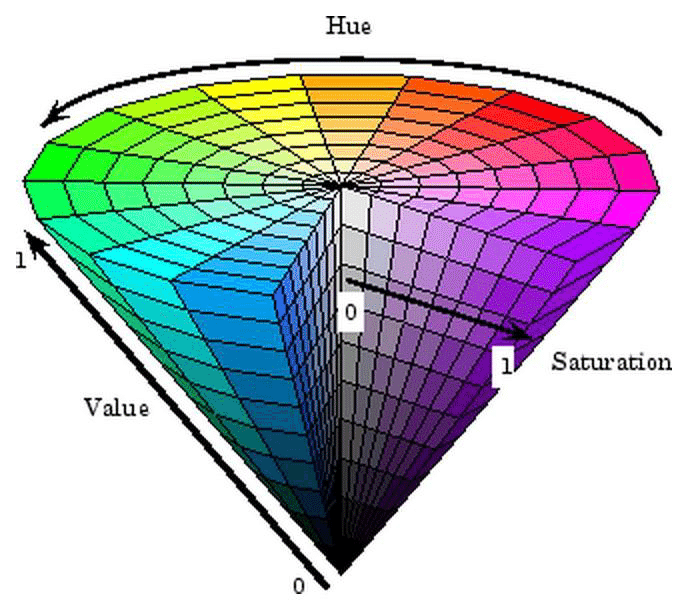
\includegraphics[width=0.5\textwidth]{figures/cv_image_formation_color_HSV.png}
			\caption{HSV color cone}
			\label{fig:rgb_color_HSV_color_cone}
		\end{subfigure}
		\begin{subfigure}[b]{0.4\textwidth}
			\centering
			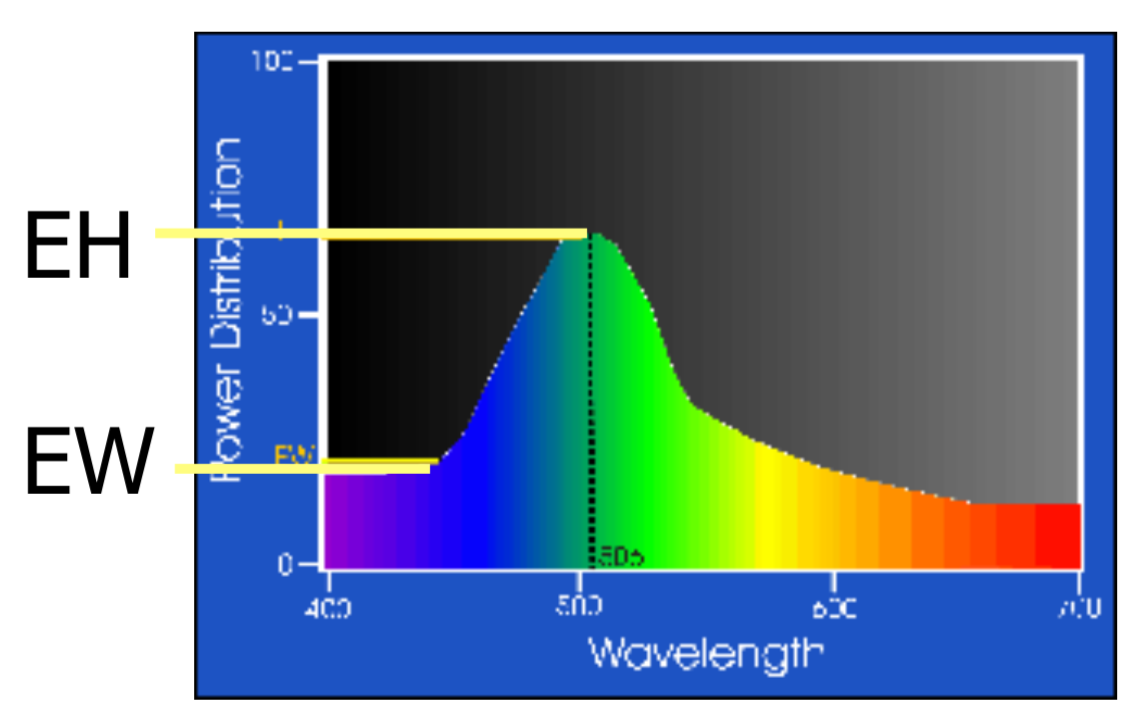
\includegraphics[width=0.6\textwidth]{figures/cv_image_formation_color_HSV_wavelength_dist.png}
			\caption{HSV wavelength distribution}
			\label{fig:rgb_color_HSV_wavelength_dist}
		\end{subfigure}
		\caption{HSV color space. }
	\end{figure}
	\item The $xy$-diagram in Figure~\ref{fig:rgb_color_wavelength_distribution_XYZ_diagram} visualizes the gamut that is visible for an average person/human vision. Different color spaces/devices capture colors by defining three points and linearly interpolate between those. However, it can be seen that there is no such gamut that can include the whole human vision gamut.
\end{itemize}
\subsection{Reflection models}
\begin{itemize}
	\item When a light source shines on an object, it might be differently perceived from different sensors/cameras although they have the same properties $\Rightarrow$ object appearance by reflectance
	\item The reflectance properties of an object/point can be specified by a \textit{BRDF}: Bi-directional reflectance distribution function $f(\theta_i, \phi_i; \theta_r, \phi_r)$ ($\theta_i$ and $\phi_i$ define the angles between input light and surface normal in $x$-$z$/$x$-$y$ direction respectively, $\theta_r$ and $\phi_r$ for the outgoing direction).
	\item A BRDF can be build up by different components, as visualized in Figure~\ref{fig:reflection_models_brdf_reflection_components}. The main parts can be distinguished into \textit{body reflection} (also referred to as mate appearance), and \textit{surface reflection} (responsible for the glossy appearance)
	\begin{figure}[ht!]
		\centering
		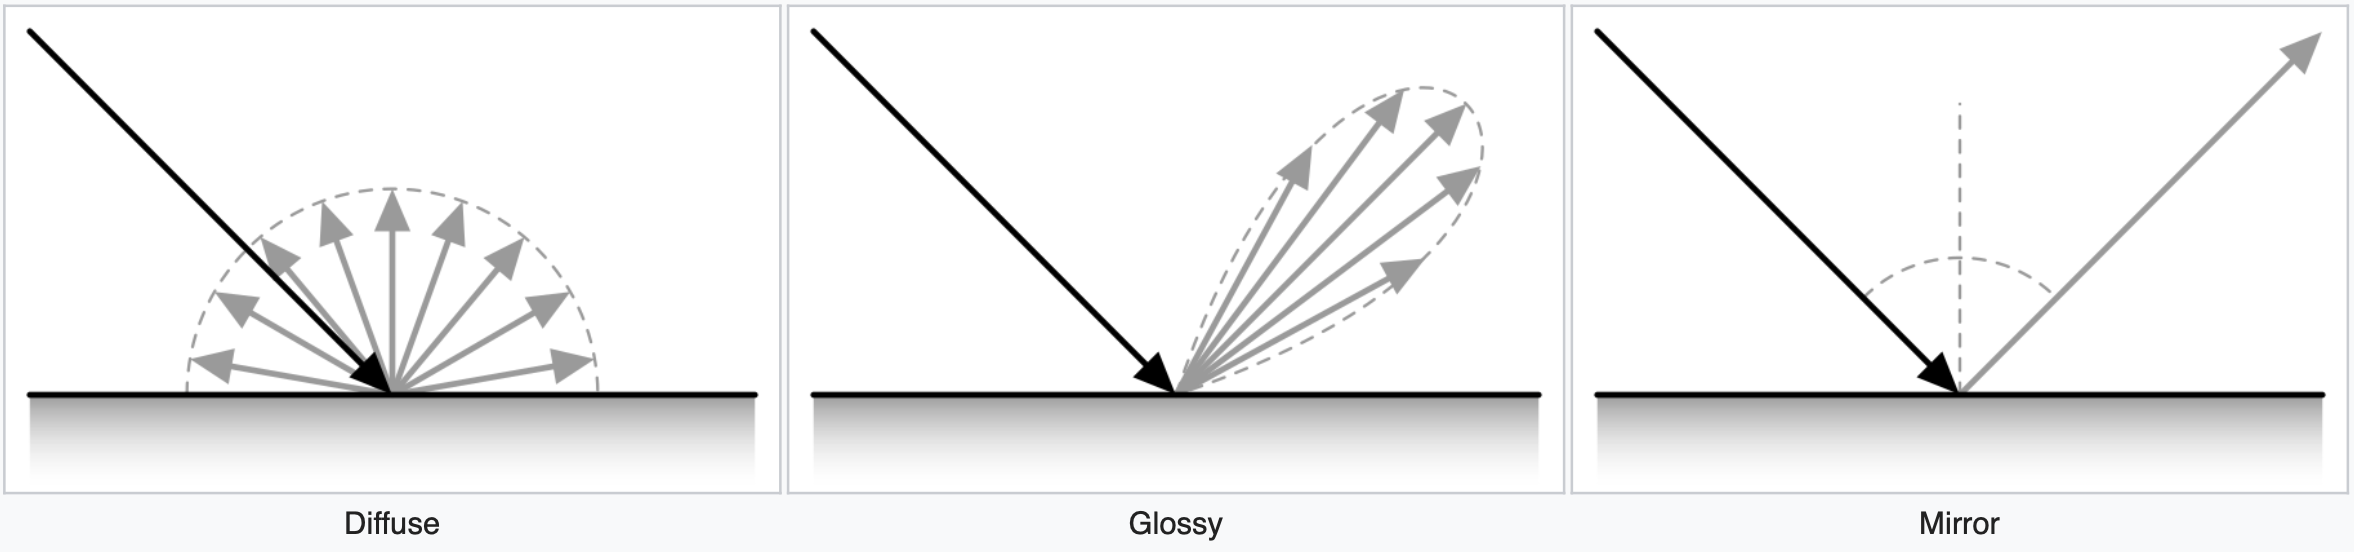
\includegraphics[width=0.8\textwidth]{figures/cv_image_formation_reflectance_properties.png}
		\caption{Different components of reflectance. Black arrow visualizes the input ray, and greyish/shaded arrows the output rays. Length of the output rays indicate their energy. }
		\label{fig:reflection_models_brdf_reflection_components}
	\end{figure}
	\item There are different models that approximate/assume/deal with certain forms of BRDFs
\end{itemize}
\subsubsection{Lambertian model}
\begin{itemize}
	\item The lambertian reflectance model assumes a BRDF that constant: $f(\theta_i, \phi_i; \theta_r, \phi_r) = \frac{\rho_d}{\pi}$ where $\rho_d$ is defined by the albedo of the object, and division of $\pi$ as energy is equally distributed over hemisphere
	\item The surface reflection/output radiance can be calculated by $L=\frac{\rho_d}{\pi}I\cos \theta_i=\frac{\rho_d}{\pi}I\cdot (\vec{n}\cdot \vec{s})$ where $I$ is light source intensity, $\vec{n}$ the surface normal and $\vec{s}$ the input ray direction.
	\item Note that the factor $(\vec{n}\cdot \vec{s})$ defines the ratio of energy/photons that interact with that point/surface
	\item By assuming a Lambertian world, we can decompose an image into a shading part (surface normals) and the albedo (reflectance) of an object.
\end{itemize}
\subsubsection{Phong model}
\begin{itemize}
	\item The Phong model extends the Lambertian model by taking glossy reflectance into account (note that mirror is mostly approximated by glossy as mirror only looks at a single output angle which is rarely met). See Figure~\ref{fig:reflection_models_phong} for the components of the Phong model
	\begin{figure}[ht!]
		\centering
		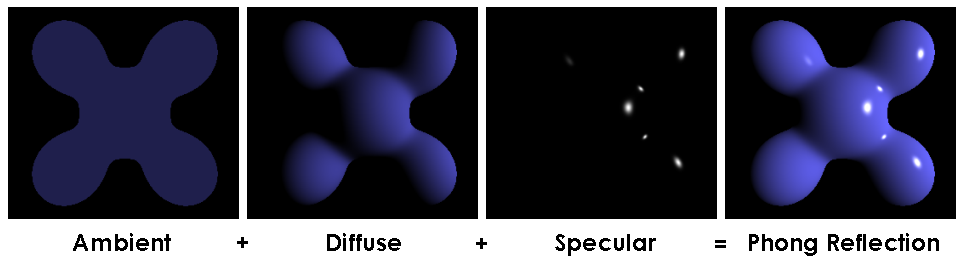
\includegraphics[width=0.7\textwidth]{figures/cv_image_formation_phong_model.png}
		\caption{The Phong model combines diffuse and glossy reflectance. Note that ambient gives the object a certain base brightness for approximating reflectance among objects/walls/...}
		\label{fig:reflection_models_phong}
	\end{figure}
	\item The reflection component of the specularity is calculated by $L_s=I\cdot \rho_s \left(\cos \phi\right)^{n_{shiny}}=I\cdot \rho_s \left(\vec{r}\cdot \vec{v}\right)^{n_{shiny}}$ where $r$ is the output ray/mirror direction (calculated by $\vec{r}=2\cdot \vec{n} \cdot (\cos \theta) - \vec{s}$), and $v$ the view direction of the sensor. 
	\item Large values for $n_{shiny}$ lead to narrow, small dot reflections (close to mirror) while small $n_{shiny}$ give broad, big surface reflectance. Note that the intensity is capped at a highest value (e.g. 1 or 255), so that multiple points can have the maximum intensity although they have a slightly different angle
	\item Also, Figure~\ref{fig:reflection_models_phong} shows that the body reflection (diffuse and ambient) contain the object color while the specularity depends on the light source (highlights color from light source)
\end{itemize}
\subsubsection{Dichromatic reflection models}
\begin{itemize}
	\item The previously discussed models only consider the light source intensity for the reflection. However, we can integrate the reflection in our color models:
	$$\text{body}_C = m_b (\vec{n}, \vec{s})  \int_\lambda e(\lambda) p(\lambda) f_C(\lambda) d\lambda$$
	$$\text{surface}_C = m_s (\vec{n}, \vec{s}, \vec{v})  \int_\lambda e(\lambda) c(\lambda) f_C(\lambda) d\lambda$$
	where $C$ is a specific channel (for example $R$, $G$ or $B$), $\vec{n}$ is the surface normal, $\vec{s}$ the input ray direction and $\vec{v}$ the viewpoint. 
	\item The function $m_b$ models the diffuse body reflection (i.e. $m_b(\vec{n}, \vec{s})=\cos \theta = \vec{n}\cdot \vec{s}$ as for Lambertian) whereas $m_s$ represents the glossy surface reflection (i.e. Phong model). 
	\item The diffuse reflectance depends on the albedo of the object $p(\lambda)$ whereas $c(\lambda)$ determines the specularity of the object for certain wavelengths.
	\item The perceived color of an object is the sum of the body and the surface
	\item Our goal is to map an input image into a space which is independent of the scene (i.e. independent of $m_b$, $m_s$, ...). Different color models can help:
	\begin{itemize}
		\item \textbf{rgb}: Assuming a white light source, normalize RGB values by the intensity (i.e. $r=\frac{R}{R+G+B}$). This leads to photometric invariance for pure matte objects ($m_b$ cancels out as it is the same for all channels when assuming $m_s=0$). Note that this approach fails if an object has no color (i.e. all gray tones are mapped to the same value).
		\item \textbf{c1c2c3}: color space is obtained from RGB manipulation and is invariant to shadowing effects of light interaction particularly for matte objects. It has similar properties as rgb, but is determined by $c_1(R,G,B) = \arctan\frac{R}{\max\left\{G,B\right\}}$
		\item \textbf{HSV} can be invariant to specularity if we assume a white light source and thus white specularity. The dominant wavelength, i.e. the hue, stays the same for those points. However, note that this model is instable for gray and especially white points that commonly occur at maximum specularity, as the hue is undefined.
		\item \textbf{l1l2l3}: Similar behavior as HSV, but calculates the values by $l_1(R,G,B) = \frac{(R-G)^2}{(R-G)^2 + (R-B)^2 + (G-B)^2}$
	\end{itemize}
	\item Figure~\ref{fig:cv_image_formation_invariance_color_spaces} summarizes some invariance properties of common color spaces
	\begin{figure}[ht!]
		\centering
		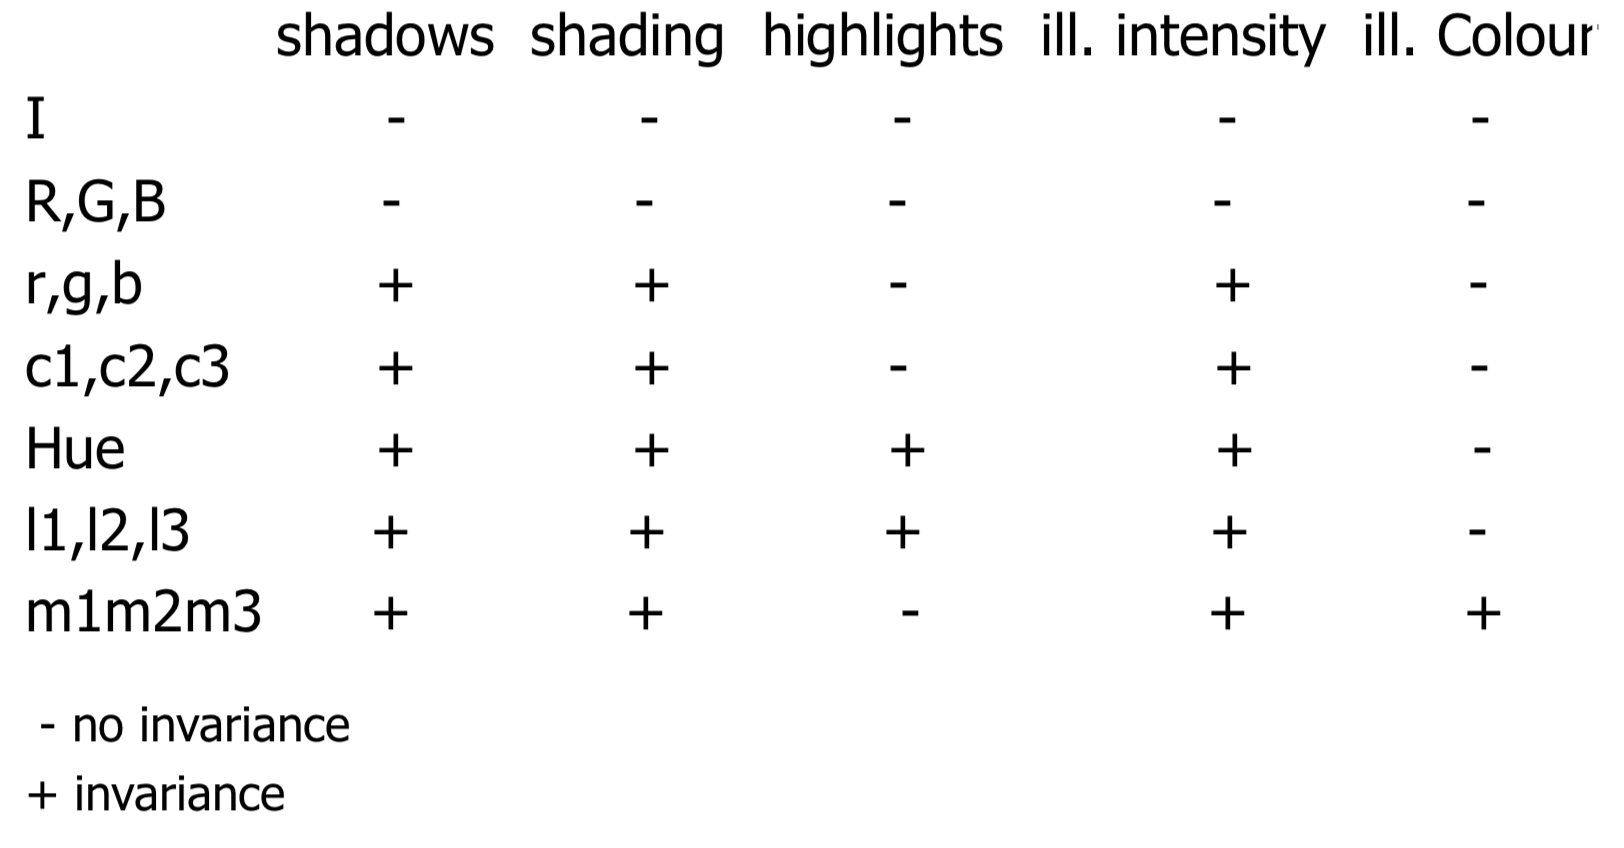
\includegraphics[width=0.5\textwidth]{figures/cv_image_formation_invariance_color_spaces.png}
		\caption{Overview of invariance in color spaces.}
		\label{fig:cv_image_formation_invariance_color_spaces}
	\end{figure}
	\item Different color spaces have different instabilities. Normalized colors get unstable around black pixels ($R=1, G=0, B=0$ is considered as pure red in rgb although in RGB it is black) whereas Hue is instable for low saturation (any hue gives same color)
	\item Another method to be invariant to shadows is filtering the image for smooth image intensity transitions as color transitions are harsh compared to that. The new image is recovered by summing up over gradients. Note that this method fails for sharp shadows and/or smooth color transitions
\end{itemize}